                %%%%%%%%%%%%%%%%%%%%%%%%%%%%%%%%%%%%%%%%%%%
                %  Template for making a very nice thesis %  
                %              		                  %  
                %    Carlos Fernando Gutiérrez Canales    % 
                %%%%%%%%%%%%%%%%%%%%%%%%%%%%%%%%%%%%%%%%%%%
\documentclass[10pt,letterpaper,twoside,openright]{report}

%Packages
%Let's call the packages
\usepackage[utf8]{inputenc}
\usepackage{babel}
\usepackage{dirtytalk}
\usepackage{epigraph}
\usepackage{mathtools}
\usepackage{float}
\usepackage{tablefootnote}
\usepackage{pdfpages}
\usepackage{array}
\usepackage{booktabs}
\usepackage{graphicx}
\usepackage{fontawesome}
\usepackage{caption}
\usepackage{subcaption}
\usepackage[round,authoryear]{natbib}
\usepackage[a4paper,width=150mm, bottom = 25mm, top = 25mm, bindingoffset = 6mm]{geometry}
%Fancy Chapter section. If you want specific configurations for your thesis, change the following lines
%The following configuration is an example of a very nice output that is really fancy and nice
\usepackage{fancyhdr}
\pagestyle{fancy}
\fancyhead{}
\fancyhead[RO,LE]{Title}
\fancyfoot{}
\fancyfoot[LE,RO]{\thepage}
\fancyfoot[LO,CE]{Chapter \thechapter}
\fancyfoot[CO,RE]{Author}
\graphicspath{{images/}}
%Hyper setup
\usepackage[breaklinks, colorlinks, urlcolor=blue, citecolor=blue, linkcolor=blue]{hyperref}
\hypersetup{
    colorlinks = true,
    linkcolor=blue,
    urlcolor=blue,
}
\usepackage{sectsty}
\sectionfont{\sffamily\large}
\subsectionfont{\sffamily\normalsize}

\renewcommand{\baselinestretch}{1.25}


%Commands created for specific reasons.
\newcommand{\pyaneti}{\href{https://github.com/oscaribv/pyaneti}{\texttt{pyaneti}\,\faGithub}}
\newcommand{\fortran}{\texttt{FORTRAN}}
\newcommand{\python}{\texttt{PYTHON}}
\newcommand{\citlalicue}{\href{https://github.com/oscaribv/citlalicue}{\texttt{citlalicue}\,\faGithub}}
\newcommand{\tesischidisima}{\href{https://github.com/Fernando-Canales/Thesis_chidisima}{\texttt{Thesis chidisima}\,\faGithub}}

%Missions
\newcommand{\kepler}{\emph{Kepler}}
\newcommand{\ktwo}{\emph{K2}}
\newcommand{\corot}{\emph{CoRoT}}
\newcommand{\plato}{\emph{PLATO}}
\newcommand{\tess}{\emph{TESS}}
\newcommand{\ariel}{\emph{ARIEL}}
\newcommand{\jwst}{\emph{JWST}}

%Physical units
\newcommand{\ms}{m\,s$^{-1}$}
\newcommand{\kms}{km\,s$^{-1}$}
\newcommand\vsini{$v$\,sin\,$i_\star$}   
\newcommand\sini{sin\,$i_\star$}   
\newcommand\vrad{$v_{\rm rad}$} 
\newcommand\vmic{$v_{\rm mic}$}
\newcommand\vmac{$v_{\rm mac}$}
\newcommand\dex{$\rm dex$}
\newcommand\teff{$T_{\rm eff}$}
\newcommand\teffo{$T_{\rm eff}$ (orig)}
\newcommand\logg{log\,{\it g$_\star$}}
\newcommand\met{[M/H]}
\newcommand{\arcsec}{''}
\newcommand{\visi}{$v$\,sin\,$i_\star$}
\newcommand{\sun}{\odot}
\newcommand\Msun{\hbox{$M_{\odot}$}}     %Msun
\newcommand\Rsun{\hbox{$R_{\odot}$}}     %Rsun
\newcommand\Mearth{\hbox{$M_{\oplus}$}}  %Mearth
\newcommand\Rearth{\hbox{$R_{\oplus}$}}  %Rearth
%\newcommand\dex{$\rm dex$}


%Journal abreviations
\newcommand{\apjl}{ApJL}
\newcommand{\apj}{ApJ}
\newcommand{\aj}{AJ}
\newcommand{\aap}{A\&A}
\newcommand{\nat}{Nature}
\newcommand{\nar}{New Astronomy Reviews}
\newcommand{\mnras}{MNRAS}
\newcommand{\araa}{ARA\&A}
\newcommand{\caa}{CAA}
\newcommand{\jcp}{Journal of Computational Physics}
\newcommand{\procspie}{Proc. SPIE 5487}
\newcommand{\pasp}{PASP}
\newcommand{\apss}{APSS}
\newcommand{\aaps}{A\&AS}
\newcommand{\apjs}{APJS}
\newcommand{\iaucirc}{IAU Circ.}
\newcommand{\aapr}{A\&ARv}
\newcommand{\actaa}{AcA}
\newcommand{\rmxaa}{Revista Mexicana de Astronom\'ia y Astrof\'isica}


\begin{document}

%Let's call the first pages of te thesis

%This line makes the first pages of the thesis to be not affected by our settings
% of the fancy packages 
\pagestyle{plain}

	%Let's put the title page
	\begin{titlepage}
    \begin{center}
        \vspace*{1cm}
        
        \Huge
        \textbf{Title}
        \vspace{1.5cm}
        
        \Large
         A Thesis presented to the\\
         \LARGE
         \textbf{Arkham Asylum}\\
        \large 
        in order to obtain the degree of\\
        \LARGE
        \textbf{Master of the League of the Shadows}\\ 
        \large
        by
        
        \LARGE
        \textbf{Author}\\
        \vfill
        \LARGE
        \textbf{Advisor:}
        \textbf{The Head of the Demon}
        
        
        \vspace{0.8cm}
        
        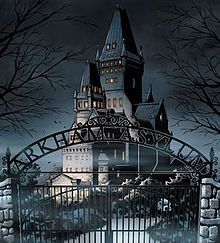
\includegraphics[width=0.4\textwidth]{images/arkham.jpg}
        
        \Large
        Arkham Asylum,\\
        Gotham City
    \end{center}
\end{titlepage}



	%Let's put the publicity here ;-)	
	\pagebreak

\vspace*{\fill}

\noindent This thesis was written using the amazing and free thesis template:
\tesischidisima.  Share/use it if you want. 

\pagebreak


	%Let's put the epigraphs
	%These are the epigraphs that I used for my Master's thesis.
\texttt{}  
\vfill
\epigraph{Like  all young  men  I set out to be  a  genius, but mercifully  laughter  intervened.}{Lawrence Durrell, Clea.}

\texttt{}  
\vfill
\epigraph{Sospecho, sin embargo, que no era muy capaz de pensar.}{Jorge Luis Borges, Funes el Memorioso.}

\texttt{}  
\vfill
\epigraph{If you hide your ignorance, no one will hit you and you will never learn.}{Ray Bradbury, Fahrenheit 451.}

\texttt{}  
\vfill
\epigraph{He sido la desesperación de mis maestros-repuso Batya-, pero al final logré aprender algo.}{Isaac Asimov, Fundación e Imperio.}


	%Lets put the abstract
	% Oscar suggests this questions to be answered in any abstrac:
 
%  What did you do? 
%  Why did you do it? What question were you trying to answer? 
%  How did you do it? State methods.
%  What did you learn? State major results. 
%  Why does it matter? Point out at least one significant implication.

\chapter*{Abstract}
...

	
	%Let's put the dedicatory
	\chapter*{Dedication}

\noindent \textbf{To Grisha}


%Let's put the table of contents
\tableofcontents

%Let's put the list of figures
\listoffigures

%Let's put the list of tables
\listoftables

%Now, let's call the main body of the thesis.

%This line makes the following pages to follow  our settings with the fancy settings. But is better to put it at the beginning of the intro.tex file
%\pagestyle{fancy}

%Let's call the Introduction
	\chapter{Introduction}
	\epigraph{No.}{William Shakespeare, Hamlet, Act III.}
	\section{Subject}


%Let's call the Second Chapter
	\chapter{Second Chapter}
	\section{Subject}

According to \cite{2021RMxAA..57..433N} and \cite{2021RNAAS...5...51B} ...


%Let's call the Conclusions
	\chapter{Conclusions}
	\section{Subject}


%Let's call the appendix
\appendix
\chapter{Appendix Name}
\section{Appendix}



%Let's call the bibliography
\bibliography{biblios/reference}
\bibliographystyle{biblios/yahapj}

\end{document}

